%!TEX root = SysSpec_ClockPendulumAnalyzer.tex
\subsection{Klassendiagramm}
Die Klassen der Software arbeiten nach dem folgenden Klassendiagramm. Es umfasst eine Implementierung der REST Definition und Klassen für die Datenbankanbindung an SQLite.
\begin{figure}[H]
    \centering
    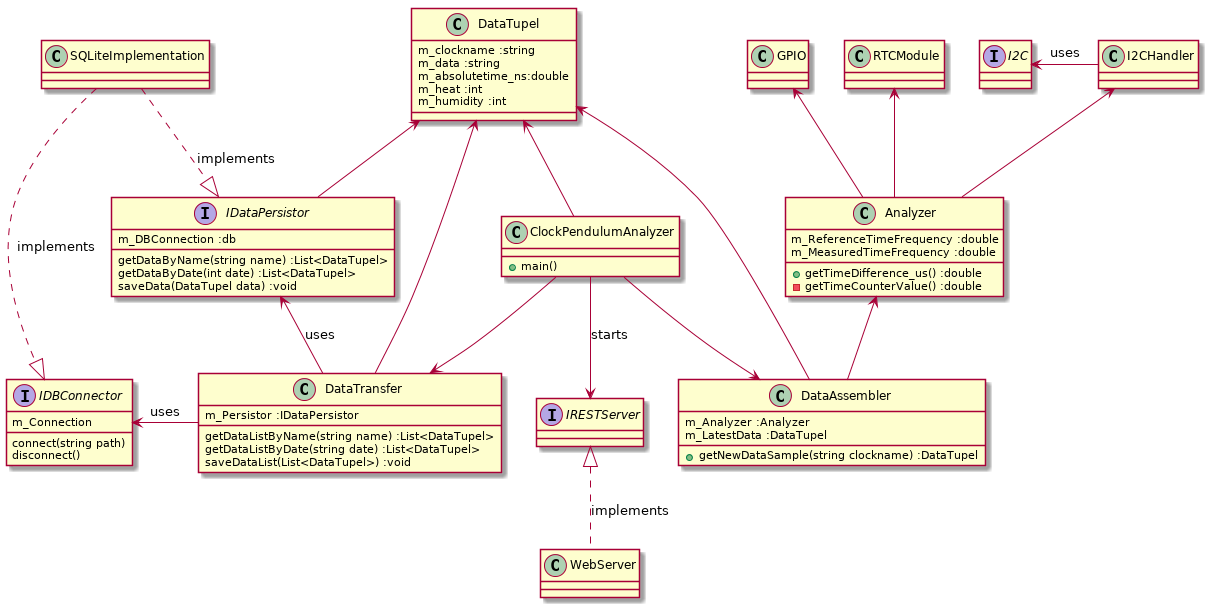
\includegraphics[width=\textwidth]{classdiagramm.png}
    \caption{Klassendiagramm der C++ Software auf dem \rpi}
\end{figure}
\subsubsection{Klassendetails}
	\begin{description}
        \item[ClockPendulumAnalyzer] Dies ist die Main Klasse. Sie startet alle Aufgaben.
        \item[GPIO] Eine Klasse die für das Arbeiten mit GPIO Pins auf dem Raspberry Pi zuständig ist.
        \item[UARTReceiver] Die Klasse läuft in einem Thread und liest die UART Verbindung. Erhaltene Nachrichten werden mittels Observer-Pattern in einer Liste gespeichert.
        \item[UARTHandler] Verbindungsaufbau und Kommunikationspunkt für UART Verbindungen. Wird vom UARTReceiver benötigt.
        \item[DataAssembler] Die Klasse ist für das Zusammenfügen von Name (aus der Main Klasse) und den einzelnen Dateninputs aus der Messung zuständig. Im Sequenzdiagramm \ref{fig:sequence_save} ist dieser Ablauf dargestellt. 
        \item[DataTransfer] Diese Klasse ist für den Transport der DataTupel zwischen Webserver, Mainklasse und Datenbank zuständig.
        \item[DataTupel] Ein Daten Transfer Objekt (DTO) als Abstraktion der gemessenen Daten zu einem gegebenen Zeitpunkt. Beinhaltet Datum+Zeit, Name, Absolut-Zeit, Referenzfrequenz und Werte für Feuchtigkeit und Wärme.
        \item[SQLiteImplementation] Die Implementierung der Schnittstelle \textit{IDataPersistor} und der \textit{IDBConnector} auf eine SQLite Umgebung.
        \item[WebServer] Implementation einer REST Schnittstelle um nach aussen die Daten zur Verfügung zu stellen (Kapitel \ref{sec:rest}).
    \end{description}
